\section{Отчёт}

За период прохождения практики был разработан прототип математической игры-головоломки, где пользователю предлагается отгадать два числа загаданных компьютером и перемноженных столбиком. Внешний вид сайта следующий:

\begin{center} 
  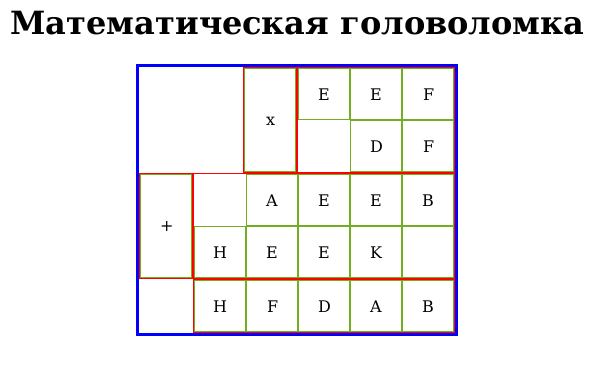
\includegraphics[width = 10cm]{img/image01.png}
\end{center}

В первой строке зашифрован первый множитель, во второй строке зашифрован второй множитель, в третьей строке зашифрован результат умножения первого множителя на цифру разряда единиц второго множителя, в четвёртой строке зашифрован результат умножения первого множителя на цифру разряда десятков второго множителя. В пятой строке зашифрован результат перемножения первого множителя на второй множитель.

Для ввода предполагаемого числа пользователю нужно нажать мышкой на соответствующую букву в результате чего на экране появится диалог ввода числа. 

\begin{center} 
  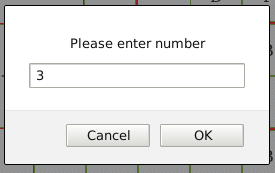
\includegraphics[width = 10cm]{img/image02.png}
\end{center}

После нажатия кнопки [OK] при совпадении введённого пользователем цифры и цифры загаданной компьютером вместо буквы будет размещена цифра.

\begin{center} 
  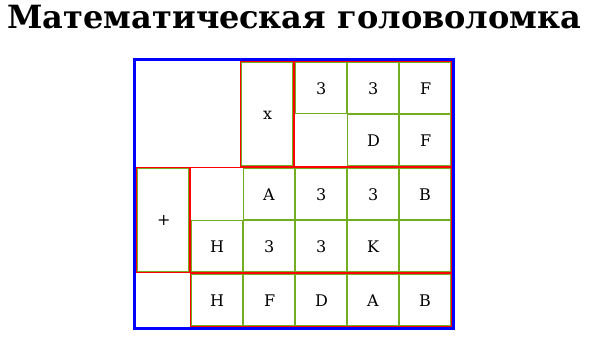
\includegraphics[width = 10cm]{img/image03.png}
\end{center}

Процесс будет повторяться до тех пор, пока не будут разгаданы все цифры. Если все цифры будут разгаданы, то выводится поздравительный диалог.

\begin{center} 
  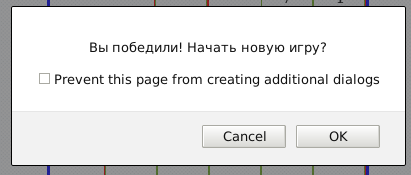
\includegraphics[width = 10cm]{img/image04.png}
\end{center}

Сайт состоит из трёх файлов: файл \verb|index.html| --- описание сайта на языке HTML, \verb|mystyle.css| --- файл с описаниями стилей (применена блочная вёрстка) и файл реализации программной части \verb|myScript.js|.

Сайт статичен, но при возникновении события окончания загрузки страницы заполняется случайно сгенерированными данными на стороне пользователя.

\pagebreak
